\chapter{Matrix-Vector Product}

When we take the product of the matrix and the vector, 
it will result in a vector. The product is a contraction 
operation, which means that the matrix's dimension reduced from two to one.
To apply the contraction, then the length of one of the matrix dimensions 
must be the same as the vector's length.

Let the $A$ be the matrix with dimensions $m$ and $n$, 
and the length of the vector $x$ be $n$.

The resultant vector $y$ will have the dimension $m$.

\vspace*{0.5 cm}
$
A = 
\begin{bmatrix}
    a_{00}  & a_{01}    & \dots     & a_{0n}\\
    a_{10}  & a_{11}    & \dots     & a_{1n}\\
    \vdots  & \vdots    & \ddots    & \vdots\\
    a_{m0}  & a_{m1}    & \dots     & a_{mn}\\
\end{bmatrix}
, x =
\begin{bmatrix}
    x_0\\
    x_1\\
    \vdots\\
    x_n\\
\end{bmatrix}
$

\begin{equation}
    y = Ax + y
    \label{eq:mtv}
\end{equation}

$
Av = 
\begin{bmatrix}
    a_{00}  & a_{01}    & \dots     & a_{0n}\\
    a_{10}  & a_{11}    & \dots     & a_{1n}\\
    \vdots  & \vdots    & \ddots    & \vdots\\
    a_{m0}  & a_{m1}    & \dots     & a_{mn}\\
\end{bmatrix}
\begin{bmatrix}
    x_0\\
    x_1\\
    \vdots\\
    x_n\\
\end{bmatrix}
=
\begin{bmatrix}
    \sum_{i=0}^na_{0i}x_i\\
    \sum_{i=0}^na_{1i}x_i\\
    \vdots\\
    \sum_{i=0}^na_{mi}x_i\\
\end{bmatrix}
$

\vspace*{0.5 cm}
The vector times matrix can calculated by taking the transpose on the both sides.
\begin{align*}
    y^T &= (Ax + y)^T\\
    y^T &= (Ax)^T + y^T\\
    y^T &= x^TA^T + y^T\\
\end{align*}

The column-major and row-major layout for the vector in the memory 
is non-distinguishable. Hence, we can use this fact and we get $x = x^T$.
If $A$ is the column-major layout then $A^T$ is the row-major layout and vice-versa.

\begin{equation}
    y = xA^T + y
    \label{eq:vtm}
\end{equation}

\clearpage
\section{Calculating Number of Operations}

Using equation \ref{eq:mtv} or \ref{eq:vtm}, we fill the below table

\begin{table}[ht]
    \centering
    \begin{tabular}{|c|c|}
        \hline
        \textbf{Name} & \textbf{Number} \\
        \hline
        Multiplication & $m$ or $n$\\
        \hline
        Addition & $m-1$ or $n-1$ \\
        \hline
    \end{tabular}
\end{table}

Total Number of Operations $=$ (Number of Multiplication $+$ Number of Addition) $\times
\begin{cases}
    n \\
    m
\end{cases}
$

Total Number of Operations $= 
\begin{cases}
    n \times (m + m - 1)\\
    m  \times (n + n - 1)
\end{cases}
$

Total Number of Operations $= 
\begin{cases}
    n \times (2m - 1)\\
    m  \times (2n - 1)
\end{cases}
$

\clearpage
\section{Performance Plots and Speedup Summary For Column-Major}

\begin{figure}[htb]
    \centering
    \caption*{Performance measurements of ?gemv implementations}
    \subfloat[\centering Single-Precision]{{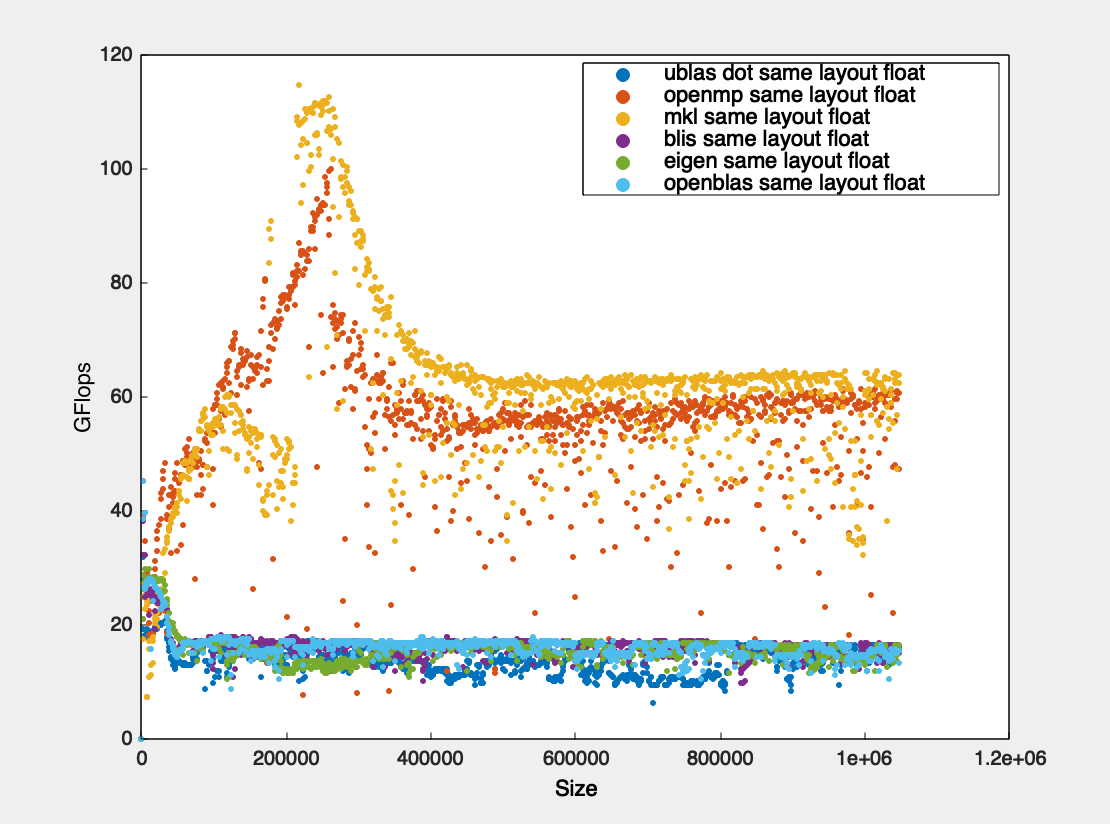
\includegraphics[width=8cm]{../assets/mtv/col_major/float_GflopsVsSize.png} }}%
    \label{fig:mtv_col_Sgflop220}
    \qquad
    \subfloat[\centering Double-Precision]{{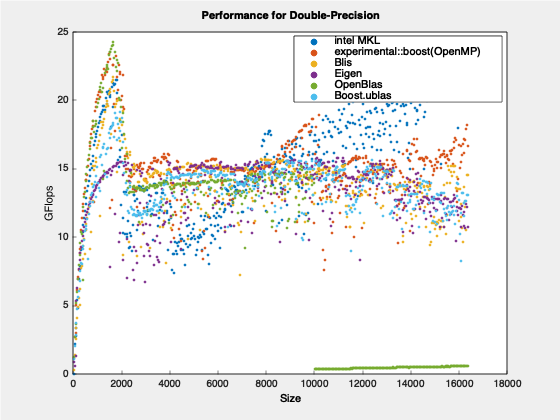
\includegraphics[width=8cm]{../assets/mtv/col_major/double_GflopsVsSize.png} }}%
    \label{fig:mtv_col_Dgflop220}
\end{figure}

\begin{figure}[htb]
    \centering
    \caption*{Sorted performance measurements of ?gemv implementations}
    \subfloat[\centering Single-Precision]{{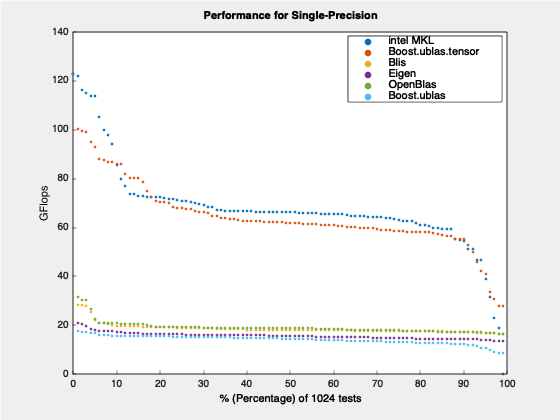
\includegraphics[width=8cm]{../assets/mtv/col_major/float_GflopsVsSize_per.png} }}%
    \label{fig:mtv_col_Sgflop_per220}
    \qquad
    \subfloat[\centering Double-Precision]{{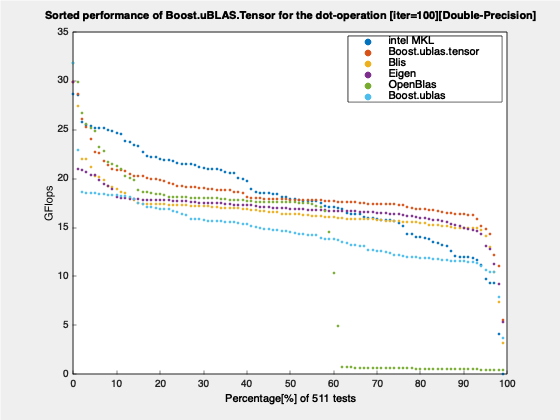
\includegraphics[width=8cm]{../assets/mtv/col_major/double_GflopsVsSize_per.png} }}%
    \label{fig:mtv_col_Dgflop_per220}
\end{figure}

\begin{figure}[htb]
    \centering
    \caption*{Comparison of the Boost.uBLAS.Tensor ?gemv implementation}
    \subfloat[\centering Single-Precision]{{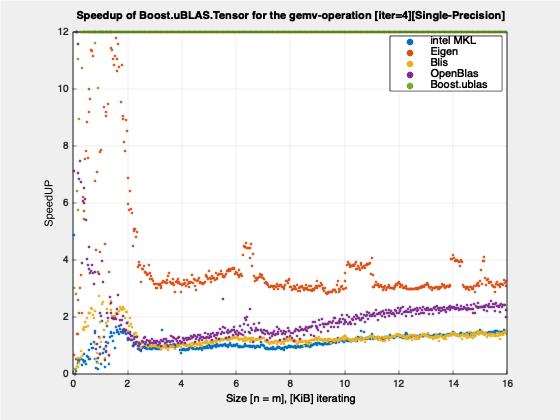
\includegraphics[width=8cm]{../assets/mtv/col_major/float_Speedup.png} }}%
    \label{fig:mtv_col_Sspeedup220}
    \qquad
    \subfloat[\centering Double-Precision]{{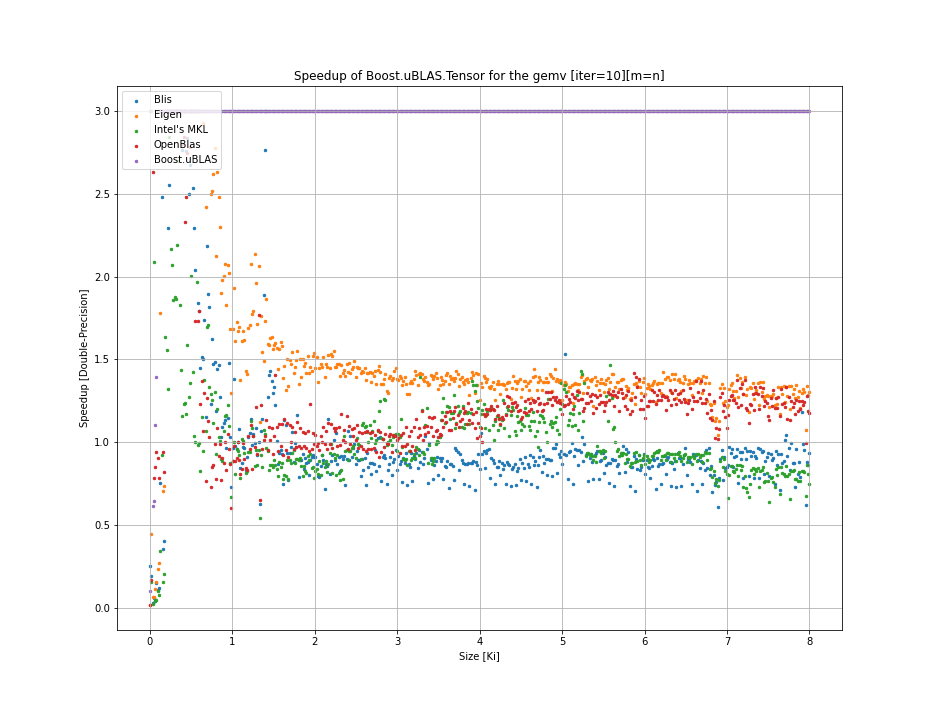
\includegraphics[width=8cm]{../assets/mtv/col_major/double_Speedup.png} }}%
    \label{fig:mtv_col_Dspeedup220}
\end{figure}

\begin{figure}[htb]
    \centering
    \caption*{Comparison of the Boost.uBLAS.Tensor ?gemv implementation [semilogy]}
    \subfloat[\centering Single-Precision]{{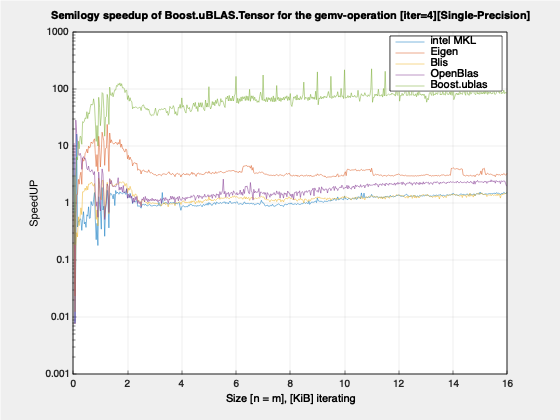
\includegraphics[width=8cm]{../assets/mtv/col_major/float_Speedup_log10.png} }}%
    \label{fig:mtv_col_Sspeedup_log10220}
    \qquad
    \subfloat[\centering Double-Precision]{{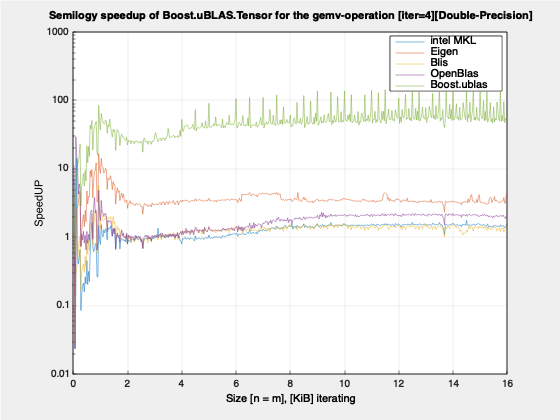
\includegraphics[width=8cm]{../assets/mtv/col_major/double_Speedup_log10.png} }}%
    \label{fig:mtv_col_Dspeedup_log10220}
\end{figure}

\begin{figure}[htb]
    \centering
    \caption*{Comparison of the Boost.uBLAS.Tensor ?gemv implementation [sorted]}
    \subfloat[\centering Single-Precision]{{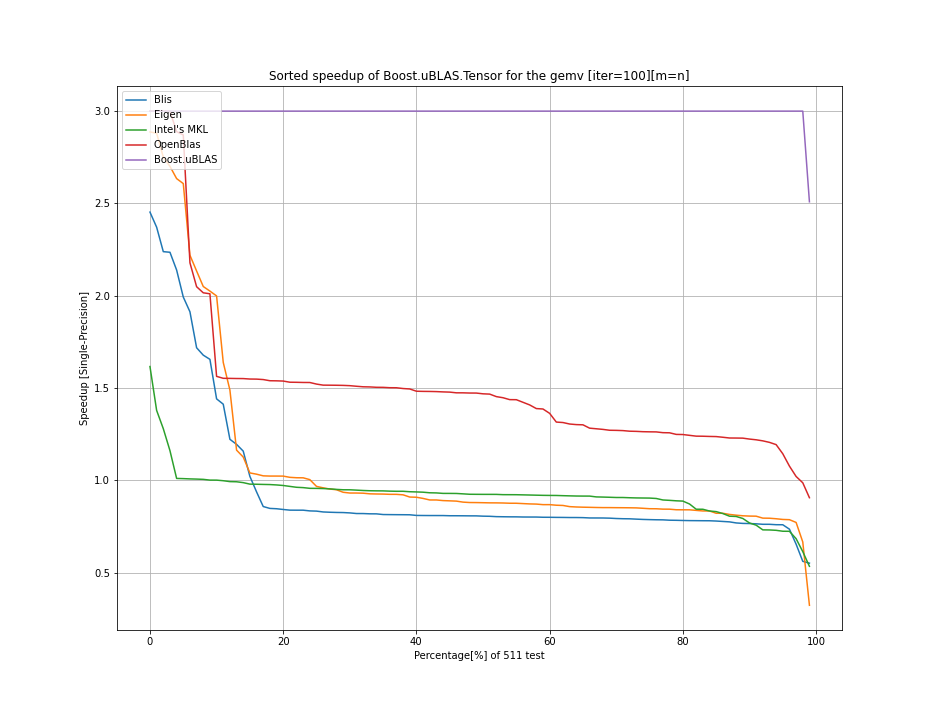
\includegraphics[width=8cm]{../assets/mtv/col_major/float_Speedup_per.png} }}%
    \label{fig:mtv_col_Sspeedup_per220}
    \qquad
    \subfloat[\centering Double-Precision]{{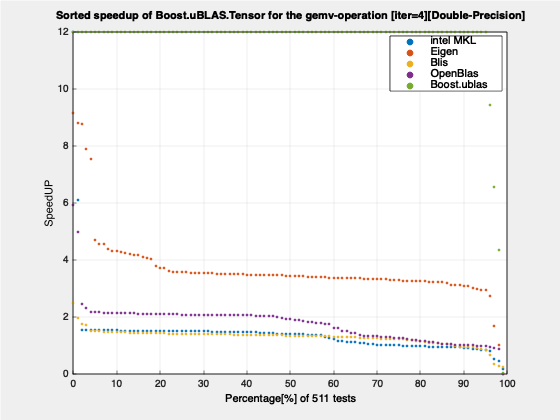
\includegraphics[width=8cm]{../assets/mtv/col_major/double_Speedup_per.png} }}%
    \label{fig:mtv_col_Dspeedup_per220}
\end{figure}

\begin{table}[ht]
    \centering
    \caption{Speedup Summary For Single-Precision}
    \begin{tabular}{|l|c|c|}
        \hline
        \textbf{Implementation} & \textbf{Speedup $\geq$ 1 [\%]} & \textbf{Speedup $\geq$ 2 [\%]}\\
        \hline
        Boost.uBLAS & $97$ & $96$ \\
        \hline
        OpenBLAS    & $93$ & $6$ \\
        \hline
        Eigen       & $96$ & $88$ \\
        \hline
        Blis        & $31$ & $7$ \\
        \hline
        Intel's MKL & $30$ & $2$ \\
        \hline
    \end{tabular}
    
    \begin{tabular}{|l|c|c|}
        \hline
        \textbf{Implementation} & \textbf{Speed-down $\geq$ 1 [\%]} & \textbf{Speed-down $\geq$ 2 [\%]}\\
        \hline
        Boost.uBLAS & $1$ & $1$ \\
        \hline
        OpenBLAS    & $5$ & $0$ \\
        \hline
        Eigen       & $2$ & $1$ \\
        \hline
        Blis        & $67$ & $1$ \\
        \hline
        Intel's MKL & $68$ & $1$ \\
        \hline
    \end{tabular}
    
    \vspace*{1 cm}

    \centering
    \caption{Speedup Summary For Double-Precision}
    \begin{tabular}{|l|c|c|}
        \hline
        \textbf{Implementation} & \textbf{Speedup $\geq$ 1 [\%]} & \textbf{Speedup $\geq$ 2 [\%]}\\
        \hline
        Boost.uBLAS & $97$ & $97$ \\
        \hline
        OpenBLAS    & $73$ & $3$ \\
        \hline
        Eigen       & $97$ & $94$ \\
        \hline
        Blis        & $53$ & $1$ \\
        \hline
        Intel's MKL & $57$ & $2$ \\
        \hline
    \end{tabular}
    
    \begin{tabular}{|l|c|c|}
        \hline
        \textbf{Implementation} & \textbf{Speed-down $\geq$ 1 [\%]} & \textbf{Speed-down $\geq$ 2 [\%]}\\
        \hline
        Boost.uBLAS & $1$ & $1$ \\
        \hline
        OpenBLAS    & $25$ & $0$ \\
        \hline
        Eigen       & $1$ & $1$ \\
        \hline
        Blis        & $45$ & $0$ \\
        \hline
        Intel's MKL & $41$ & $1$ \\
        \hline
    \end{tabular}
\end{table}

\clearpage
\section{Performance Metrics For Column-Major}

\subsection*{Range[Start: $32$, End: $16382$, Step: $32$]}

\begin{table}[ht]
    \centering
    \caption{GFLOPS For Single-Precision}
    \begin{tabular}{|l|c|c|}
        \hline
        \textbf{Implementation} & \textbf{Max} & \textbf{Average}\\
        \hline
        Boost.uBLAS.Tensor  & $66.6854$& $13.688$ \\
        \hline
        Boost.uBLAS         & $2.19943$& $0.377742$ \\
        \hline
        Intel's MKL         & $87.1418$& $15.2925$ \\
        \hline
        OpenBLAS            & $29.1065$& $9.17016$ \\
        \hline
        Blis                & $27.9843$& $12.2749$ \\
        \hline
        Eigen               & $12.091$& $3.87655$ \\
        \hline
    \end{tabular}

    \vspace*{1 cm}

    \centering
    \caption{GFLOPS For Double-Precision}
    \begin{tabular}{|l|c|c|}
        \hline
        \textbf{Implementation} & \textbf{Max} & \textbf{Average}\\
        \hline
        Boost.uBLAS.Tensor  & $32.5937$ & $5.93336$ \\
        \hline
        Boost.uBLAS         & $1.55798$ & $0.257134$ \\
        \hline
        Intel's MKL         & $36.9107$ & $6.73425$ \\
        \hline
        OpenBLAS            & $12.5549$ & $4.72732$ \\
        \hline
        Blis                & $13.7302$ & $5.72709$ \\
        \hline
        Eigen               & $4.92076$ & $1.98264$ \\
        \hline
    \end{tabular}
\end{table}

\begin{table}[ht]
    \centering
    \caption{Utilization[\%] For Single-Precision}
    \begin{tabular}{|l|c|c|}
        \hline
        \textbf{Implementation} & \textbf{Max} & \textbf{Average}\\
        \hline
        Boost.uBLAS.Tensor  & $11.3256$& $2.32473$ \\
        \hline
        Boost.uBLAS         & $0.373545$& $0.0641546$ \\
        \hline
        Intel's MKL         & $14.7999$& $2.59723$ \\
        \hline
        OpenBLAS            & $4.94337$& $1.55743$ \\
        \hline
        Blis                & $4.75276$& $2.08474$ \\
        \hline
        Eigen               & $2.0535$& $0.658382$ \\
        \hline
    \end{tabular}

    \vspace*{1 cm}

    \centering
    \caption{Utilization[\%] For Double-Precision}
    \begin{tabular}{|l|c|c|}
        \hline
        \textbf{Implementation} & \textbf{Max} & \textbf{Average}\\
        \hline
        Boost.uBLAS.Tensor  & $11.0712$ & $2.01541$ \\
        \hline
        Boost.uBLAS         & $0.529206$ & $0.0873417$ \\
        \hline
        Intel's MKL         & $12.5376$ & $2.28745$ \\
        \hline
        OpenBLAS            & $4.26458$ & $1.60575$ \\
        \hline
        Blis                & $4.66377$ & $1.94534$ \\
        \hline
        Eigen               & $1.67146$ & $0.67345$ \\
        \hline
    \end{tabular}
\end{table}

\begin{table}[ht]
    \centering
    \caption{Speedup(Boost.uBLAS.Tensor) For Single-Precision}
    \begin{tabular}{|l|c|c|}
        \hline
        \textbf{Implementation} & \textbf{Max} & \textbf{Average}\\
        \hline
        Boost.uBLAS         & $30.3194$ & $36.2364$ \\
        \hline
        Intel's MKL         & $0.765251$ & $0.895079$ \\
        \hline
        OpenBLAS            & $2.29108$ & $1.49267$ \\
        \hline
        Blis                & $2.38296$ & $1.11512$ \\
        \hline
        Eigen               & $5.51529$ & $3.53098$ \\
        \hline
    \end{tabular}

    \vspace*{1 cm}

    \centering
    \caption{Speedup(Boost.uBLAS.Tensor) For Double-Precision}
    \begin{tabular}{|l|c|c|}
        \hline
        \textbf{Implementation} & \textbf{Max} & \textbf{Average}\\
        \hline
        Boost.uBLAS         & $20.9205$ & $23.075$ \\
        \hline
        Intel's MKL         & $0.883043$ & $0.881072$ \\
        \hline
        OpenBLAS            & $2.59609$ & $1.25512$ \\
        \hline
        Blis                & $2.37388$ & $1.03602$ \\
        \hline
        Eigen               & $6.62371$ & $2.99266$ \\
        \hline
    \end{tabular}
\end{table}